\section{Übertragungsmedien}
    \subsubsection{Signale}
    \begin{formula}{Ausbreitungsgeschwindigkeit}\\
        Lichtgeschwindigkeit im Vakuum: $c_0 = 299'792'458 m/s$\\
        $$C_{Medium} = 200'000 km/s \approx 2/3 c_0$$
    \end{formula}

    \begin{formula}{Signaldämpfung} Leistungsabnahme auf Übertragungsstrecke\\
        $P_1$: Anfangsleistung, $P_2$: Leistung am Ende der Strecke
        $$Signaldämpfung[dB] = 10 \cdot log (\frac{P_1}{P_2}) = 10 \cdot log((\frac{U_1}{U_2})^2) = 20 \cdot log(\frac{U_1}{U_2})$$
        \includegraphics[width=1\linewidth]{images/Signaldämpfung.png}\\
        Halbierung der Leistung entspricht ca. 3dB
    \end{formula}    

    \begin{formula}{SNR} Signal to Noise Ratio
        $$SNR_{dB} = 10 \cdot log(\frac{P_{Signal}}{P_{Störung}}) = 20 \cdot log(\frac{U_{Signal}}{U_{Störung}})$$
    \end{formula}
    
    \begin{definition}{Dämpfungsbelag}Dämpfung pro Distanz - dB pro 100m
        \begin{center}
            \includegraphics[width=0.9\linewidth]{images/Dämpfungsbelag_Kabel.png}
        \end{center}
    \end{definition}

    \begin{concept}{Leistungslänge Bandbreite und Dämpfungsbelag}
        \begin{itemize}
            \item maximale Leitungslänge $L_{max}$:
            $$L_{max} = \frac{SNR_{min}}{Dämpfungsbelag}$$
            $SNR_{min}$: Minimales benötigtes SNR für korrekte Datenübertragung
            \item tiefere Bitrate $\rightarrow$ grössere Distanzen können erreicht werden
            \item Die Bandbreite (Frequenz) ist abhängig zum Dämpfungsbelag.
            \item höhere Kabelkategorien haben bessere Schirmung $\rightarrow$ tolerieren höhere Dämpfung
        \end{itemize}
    \end{concept}

    

    \subsubsection{Kabeltypen}
    \begin{concept}{Overview}
        \begin{itemize}
            \item Koaxialkabel: Geeignet für hochfrequente Signale
            \item Twinaxialkabel: Hoher Schutz (double koax)
            \item Twisted Pair (TP): Häufig im Einsatz (Shielded/Unshielded)
            \item Glasfaser: Hohe Bandbreite, Geringe Dämpfung, resistent
                \begin{itemize}
                    \item Multimode, Singlemode (besser)
                \end{itemize}
        \end{itemize}        
    \end{concept}

    \begin{definition}{Paarsymmetrische Kabel (Twisted Pair)}
        \begin{itemize}
            \item Schirmeigenschaften
            \begin{itemize}
                \item Drahtgeflecht: niederfrequente Einstreuungen
                \item metallisch beschichtete Folien: hochfrequente Störungen
            \end{itemize}
            \item Bezeichnungsschema ISO/IEC 11801\\
            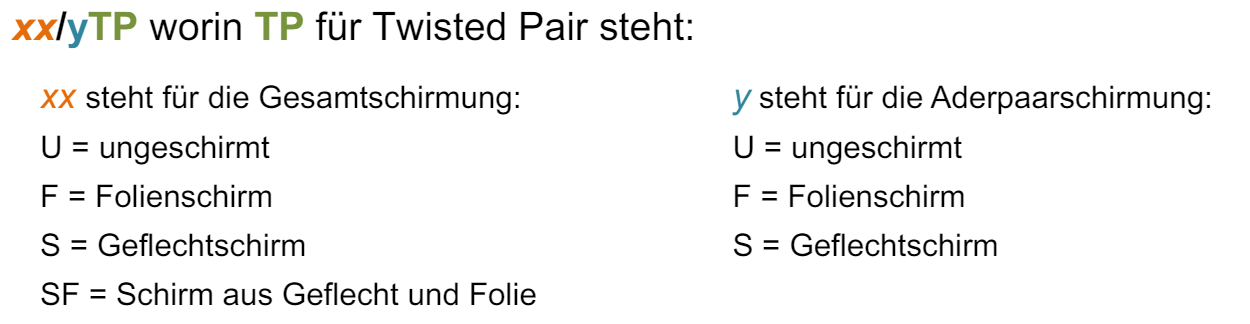
\includegraphics[width=\linewidth]{images/STP_Schirmeigenschaften.png}
        \end{itemize}
        Behebung von Störungen (crosstalk):
        \begin{itemize}
            \item Kapazitiv: Komplementäres Signal, elektrisch leitenden Schirm
            \item Induktiv: Verdrillte Aderpaare
        \end{itemize}
    \end{definition}

    

    
        
    